\documentclass[12pt, titlepage]{article}

\usepackage{fullpage}
\usepackage[round]{natbib}
\usepackage{multirow}
\usepackage{booktabs}
\usepackage{tabularx}
\usepackage{graphicx}
\usepackage{float}
\usepackage{hyperref}
\hypersetup{
    colorlinks,
    citecolor=blue,
    filecolor=black,
    linkcolor=red,
    urlcolor=blue
}
\usepackage{subfig}

%% Comments

\usepackage{color}

\newif\ifcomments\commentstrue %displays comments
%\newif\ifcomments\commentsfalse %so that comments do not display

\ifcomments
\newcommand{\authornote}[3]{\textcolor{#1}{[#3 ---#2]}}
\newcommand{\todo}[1]{\textcolor{red}{[TODO: #1]}}
\else
\newcommand{\authornote}[3]{}
\newcommand{\todo}[1]{}
\fi

\newcommand{\wss}[1]{\authornote{blue}{SS}{#1}} 
\newcommand{\plt}[1]{\authornote{magenta}{TPLT}{#1}} %For explanation of the template
\newcommand{\an}[1]{\authornote{cyan}{Author}{#1}}

%% Common Parts

\newcommand{\progname}{REVITALIZE} % PUT YOUR PROGRAM NAME HERE
\newcommand{\authname}{Team 13, REVITALIZE
\\ Bill Nguyen
\\ Syed Bokhari
\\ Hasan Kibria
\\ Youssef Dahab
\\ Logan Brown
\\ Mahmoud Anklis} % AUTHOR NAMES                  

\usepackage{hyperref}
    \hypersetup{colorlinks=true, linkcolor=blue, citecolor=blue, filecolor=blue,
                urlcolor=blue, unicode=false}
    \urlstyle{same}
                                


\newcounter{acnum}
\newcommand{\actheacnum}{AC\theacnum}
\newcommand{\acref}[1]{AC\ref{#1}}

\newcounter{ucnum}
\newcommand{\uctheucnum}{UC\theucnum}
\newcommand{\uref}[1]{UC\ref{#1}}

\newcounter{mnum}
\newcommand{\mthemnum}{M\themnum}
\newcommand{\mref}[1]{M\ref{#1}}

\begin{document}

\title{System Design for \progname{}} 
\author{\authname}
\date{\today}

\maketitle

\pagenumbering{roman}

\section{Revision History}

\begin{tabularx}{\textwidth}{p{3cm}p{2cm}X}
\toprule {\bf Date} & {\bf Version} & {\bf Notes}\\
\midrule
January 18th, 2023 & Syed Bokhari & Added user interface figma sketches\\
January 18th, 2023 & Syed Bokhari & Added interface descriptions and additional information\\
January 18th, 2023 & Syed Bokhari & Added reflection question answers\\
\bottomrule
\end{tabularx}

\newpage

\section{Reference Material}

This section records information for easy reference.

\subsection{Abbreviations and Acronyms}

\renewcommand{\arraystretch}{1.2}
\begin{tabular}{l l} 
  \toprule		
  \textbf{symbol} & \textbf{description}\\
  \midrule 
  \progname & Explanation of program name\\
  \wss{...} & \wss{...}\\
  \bottomrule
\end{tabular}\\

\newpage

\tableofcontents

\newpage

\listoftables

\listoffigures

\newpage

\pagenumbering{arabic}

\section{Introduction}

\wss{Include references to your other documentation}

\section{Purpose}

\wss{Purpose of your design documentation}

\wss{Point to your other design documents}

\section{Scope}

\wss{Include a figure that show the System Context (showing the boundary between
your system and the environment around it.)}

\section{Project Overview}

\subsection{Normal Behaviour}

\subsection{Undesired Event Handling}

\wss{How you will approach undesired events}

\subsection{Component Diagram}

\subsection{Connection Between Requirements and Design} \label{SecConnection}

\wss{The intention of this section is to document decisions that are made
  ``between'' the requirements and the design.  To satisfy some requirements,
  design decisions need to be made.  Rather than make these decisions implicit,
  they are explicitly recorded here.  For instance, if a program has security
  requirements, a specific design decision may be made to satisfy those
  requirements with a password.}

\section{System Variables}

\wss{Include this section for Mechatronics projects}

\subsection{Monitored Variables}

\subsection{Controlled Variables}

\subsection{Constants Variables}

\section{User Interfaces}

\begin{figure}[H]%
    \centering
    \subfloat[\centering Start]{{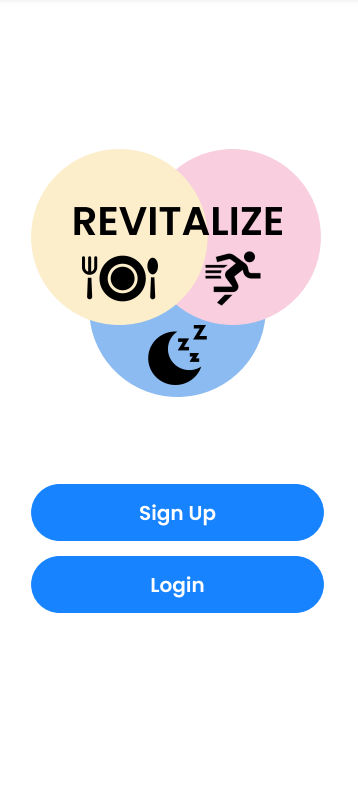
\includegraphics[width=5cm]{revitalize_figma_sketches/p1.png} }}%
    \subfloat[\centering Signup]{{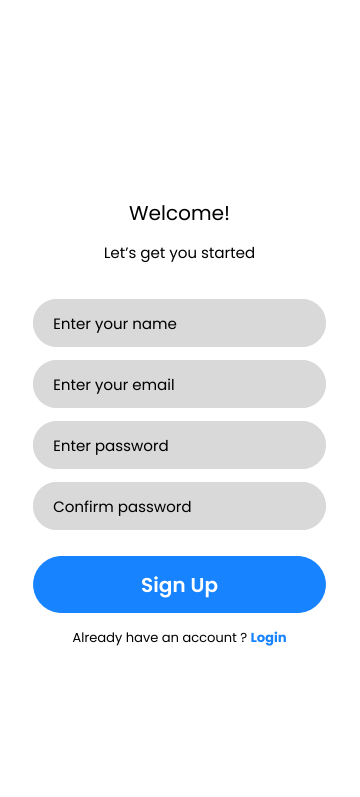
\includegraphics[width=5cm]{revitalize_figma_sketches/p2.png} }}%
    \subfloat[\centering Login]{{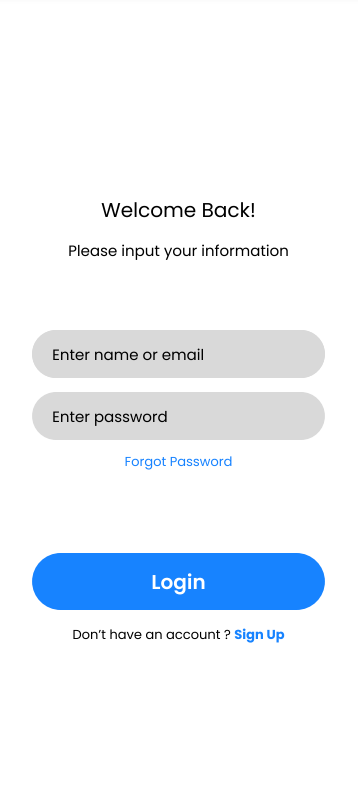
\includegraphics[width=5cm]{revitalize_figma_sketches/p3.png} }}%
    \label{fig:example}%
\end{figure}

\begin{figure}[H]%
    \centering
    \subfloat[\centering Main]{{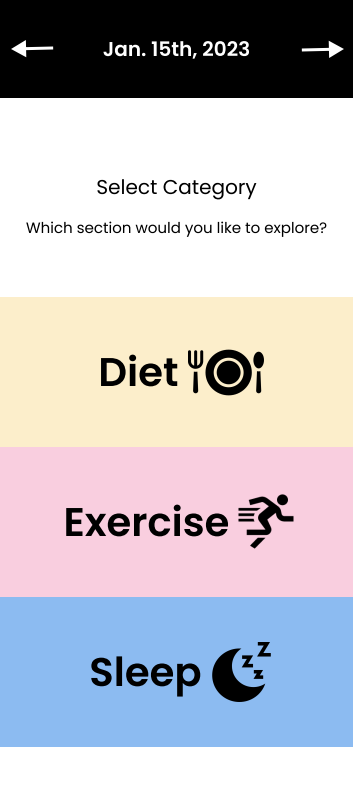
\includegraphics[width=5cm]{revitalize_figma_sketches/p4.png} }}%
    \subfloat[\centering Diet Main]{{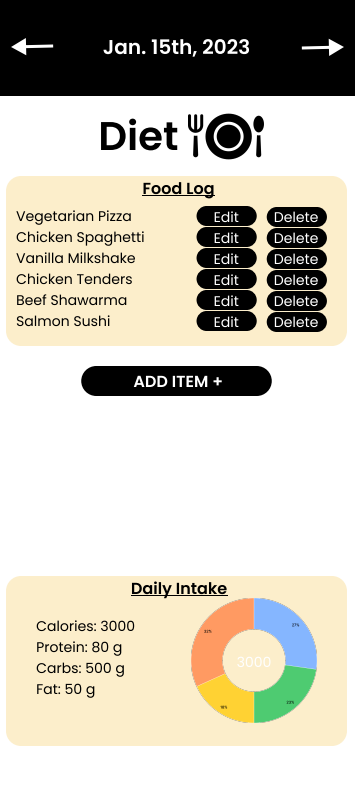
\includegraphics[width=5cm]{revitalize_figma_sketches/p5.png} }}%
    \subfloat[\centering Diet Search/Add Custom Meal]{{
\includegraphics[width=5cm]{revitalize_figma_sketches/p6.png} }}%
    \label{fig:example}%
\end{figure}

\begin{figure}[H]%
    \centering
    \subfloat[\centering Diet Add Custom Meal]{{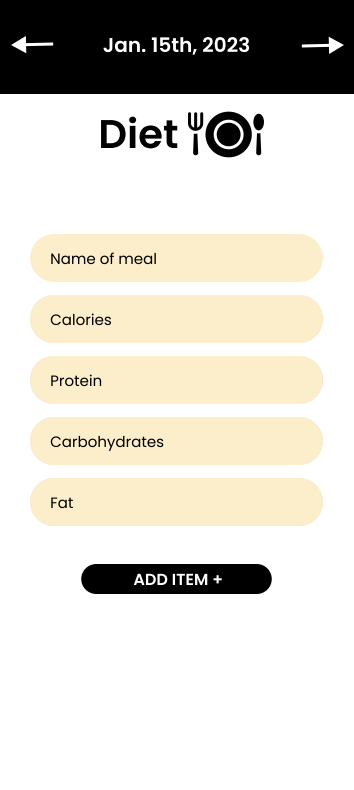
\includegraphics[width=5cm]{revitalize_figma_sketches/p7.png} }}%
    \subfloat[\centering Diet Recipe Search]{{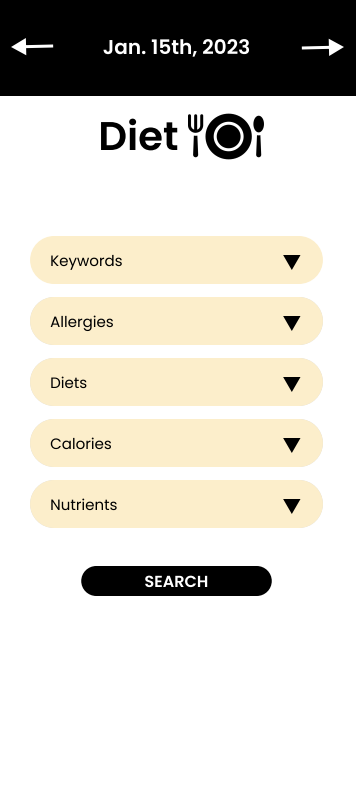
\includegraphics[width=5cm]{revitalize_figma_sketches/p8.png} }}%
    \subfloat[\centering Diet Recipe List]{{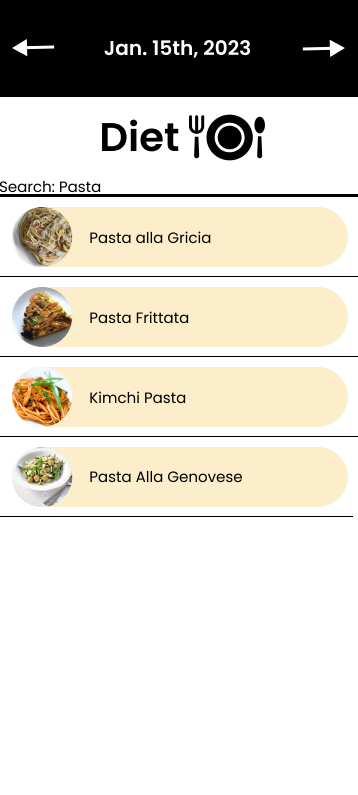
\includegraphics[width=5cm]{revitalize_figma_sketches/p9.png} }}%
    \label{fig:example}%
\end{figure}

\begin{figure}[H]%
    \centering
    \subfloat[\centering Diet Recipe Info]{{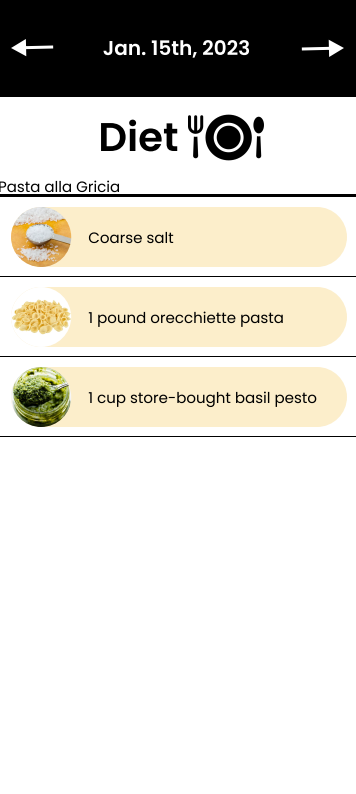
\includegraphics[width=5cm]{revitalize_figma_sketches/p10.png} }}%
    \subfloat[\centering Exercise Main]{{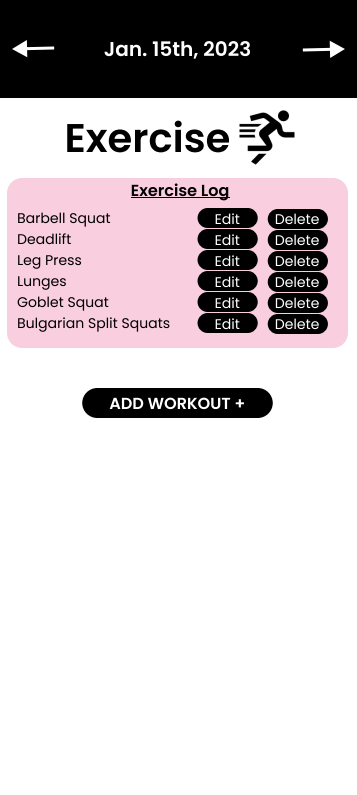
\includegraphics[width=5cm]{revitalize_figma_sketches/p11.png} }}%
    \subfloat[\centering Exercise List]{{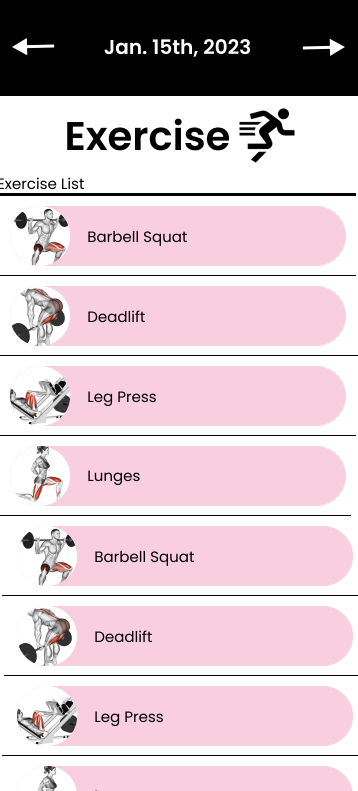
\includegraphics[width=5cm]{revitalize_figma_sketches/p12.png} }}%
    \label{fig:example}%
\end{figure}

\begin{figure}[H]%
    \centering
    \subfloat[\centering Exercuse Details]{{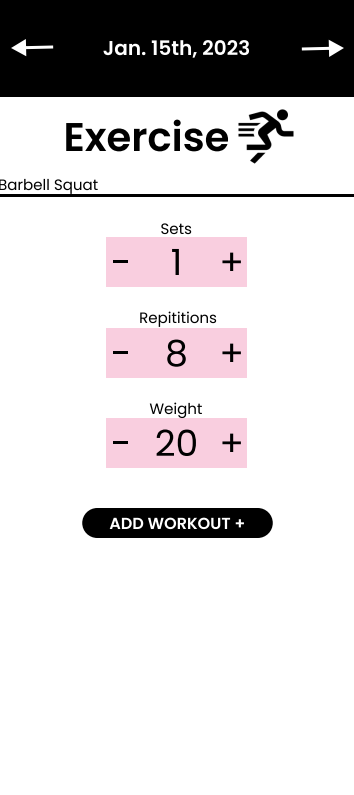
\includegraphics[width=5cm]{revitalize_figma_sketches/p13.png} }}%
    \subfloat[\centering Sleep]{{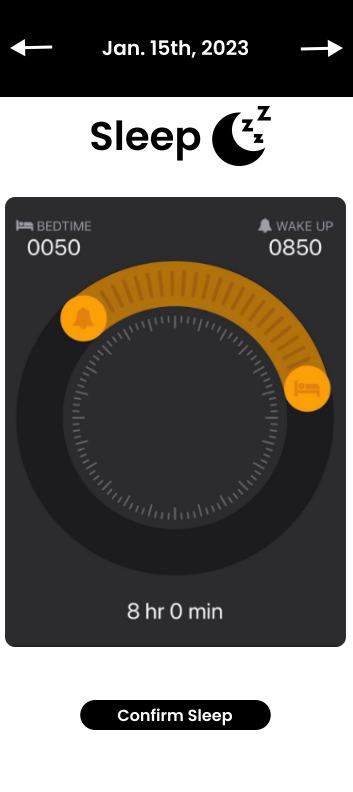
\includegraphics[width=5cm]{revitalize_figma_sketches/p14.png} }}%
    \label{fig:example}%
\end{figure}


\section{Design of Hardware}

\wss{Most relevant for mechatronics projects}
\wss{Show what will be acquired}
\wss{Show what will be built, with detail on fabrication and materials}
\wss{Include appendices as appropriate, possibly with sketches, drawings, CAD, etc}

\section{Design of Electrical Components}

\wss{Most relevant for mechatronics projects}
\wss{Show what will be acquired}
\wss{Show what will be built, with detail on fabrication and materials}
\wss{Include appendices as appropriate, possibly with sketches, drawings,
circuit diagrams, etc}

\section{Design of Communication Protocols}

\wss{If appropriate}

\section{Timeline}

\wss{Schedule of tasks and who is responsible}

% \bibliographystyle {plainnat}
% \bibliography{../../../refs/References}

\newpage{}

\appendix

\section{Interface}

figure (a): This is the start screen when launching the application. It offers the user the ability to either sign up or login.
\\figure (b): This is the signup screen. The user must input valid information and register with confirmation from the database.
\\figure (c): This is the login screen. The user must input valid credentials to successfully enter the main screen.
\\figure (d): This is the main screen. The user can select from the three application categories and enter their specific page after click. The user can select the calender value and change the date accordingly to see the information for the given day.
\\figure (e): This is the diet main screen. The food log is available to view and each entry can be edited or deleted. On the bottom of the screen, the total statistics of the day can be seen. The add item button is clicked to go to figure (f).
\\figure (f): This is the screen to traverse to the search or add custom meal pages.
\\figure (g): This is the custom meal screen. The user can input custom information to add to the food log.
\\figure (h): This is the recipe search screen. The user can select the API query options from the drop down to construct a unique recipe list.
\\figure (i): This is the recipe list screen. The recipes are listed based on the previous page query. 
\\figure (j): This is the recipe information screen. Specific information relating to incredients for each recipe is listed.
\\figure (k): This is the exercise main screen. It displays a list of exercises for the day that can be edited or deleted. A workout can be added by clicking the button.
\\figure (l): This is the exercise list screen.The screen displays a list of exercises available through the API. Once selected, the user is taken to figure m where they can add the custom information for their exercise. 
\\figure (m): This is the execise details screen. The user can customize their sets, reps and weight for accurate tracking.
\\figure (n): This is the sleep screen. The user can alter the clock value if the API sleep tracking was not correct and they can confirm the entry to add to their sleep log. 

\section{Mechanical Hardware}

\section{Electrical Components}

\section{Communication Protocols}

\section{Reflection}

The information in this section will be used to evaluate the team members on the
graduate attribute of Problem Analysis and Design.  Please answer the following questions:

\begin{enumerate}
  \item What are the limitations of your solution?  Put another way, given
  unlimited resources, what could you do to make the project better? (LO\_ProbSolutions)
	
\textbf{Syed}: Our main features are reliant on the database provided by external APIs. The recipe list and the exercise list can only give the user's the information that is accessable through the API. This limits the design of the app due to the limited query information. \\
\textbf{Bill}: Project does not have functionalities such as analytics of data and predictive models that can potentially benefit the user experience. \\
\textbf{Hasan}: Since time is a key resource, unlimited resources would imply unlimited time. I think with unlimited (or rather plenty of) time, we could improve every aspect- from the documentation to the UI to the business logic. \\
  \item Give a brief overview of other design solutions you considered.  What
  are the benefits and tradeoffs of those other designs compared with the chosen
  design?  From all the potential options, why did you select documented design?
  (LO\_Explores)

\textbf{Syed}: We considered a self serving exercise list, where the user would be able to add their own custom exercises. This seemed like a great option for user customizability, however the tradeoff is that the user must spend a tedious amount of time inputting the information. Instead, we have a preset list of the most common exercises that the user can quickly select and add their sets, repititions and weight. \\
\textbf{Bill}: We considered using analytics to find statisctics and trends of which features are used the most/the least etc. which could help us improve user experience. Also considered using predictive models such as giving recipe/exercise suggestions to user based on user data. These were great options, but are options that are nice to have and were considered stretch goals. \\
\textbf{Hasan}: To be honest I do not completely remember all the other design solutions we covered. However, I do remember that this design solution stood out because it solved a real problem; ie. an all-in-one health application that is user friendly and easily learned. \\
\end{enumerate}

\end{document}